\chapter{Design}
\label{ch:kap4}

\section{Concept Art}
\label{ConceptArt}
The concept artists main assignments where making the concept art for the character, the environment and the UI elements. There's a 3D universe which is made up to look like it is build with pieces of cardboard.

\subsection{Characters}
\label{Characters}
\cite{DynamicCharacters}

\subsection{Environment}
\label{Environment}

\section{Game Design}
\label{GameDesign}

\subsection{Level Design}
\label{LevelDesign}

\subsection{Type of Game}

\subsection{Failing the Game}
Everyday people all over the world plays Video Games, hundreds of millions of them and most of them will experience failure while playing. We humans have a desire to succeed and to feel competent, but the game players choose to play and engage in, is an activity in which they are almost certain to fail. They end up with this feeling of of being incompetent, but because of \textit{The Paradox of Failing} in games, we know that player actually prefer games in which they fail in.\cite[P.~2]{TheArtOfFailure}.

\textit{The Paradox of Failing} in games can be declared as:
\begin{itemize}
    \item We as humans in general avoid failure.
    \item We often experience failure while playing games.
    \item We look for games, even though we will almost certainly experience that we would normally avoid. 
\end{itemize}

This paradox, may be some of the reasons why we seek out something that could leave us with the feeling of sadness, fear or even disgust. There is this conundrum here, which is that we usually try to avoid negative and unpleasant emotions, yet we seek out these emotions in films, stories, games and art.\cite[P.~2-4]{TheArtOfFailure}

When you fail in a game, that means in some way you were inadequate. That feeling of inadequacy is not pleasant for us, however it motivates us to keep trying, to play more in order to get away from the same feeling of inadequacy and failure. This is done often by improving our skills, games promise us a change to redeem our self and this is what distinguishes failure in game from failure in our real life.
\cite[P.~7]{TheArtOfFailure}.

The feeling of failure can be a challenging emotion for children to deal with, fortunately there is books out there that explains it. There is this book called \textit{Liam Wins the Game, Sometimes} written by Jane Whelen Banks, that teaches children how to deal with the feeling of winning or losing a game. The author tells the children that the feeling of disappointment is okay and acceptable when loosing a game. Throwing a tantrum on the other hand is not okay and is unacceptable when loosing a game.\cite[P.~8]{TheArtOfFailure}.

In the field of game studies, \textit{Game Playing} has been described as entering a \textit{``Entering a Magic Circle"} by Eric Zimmerman and Katie Salen. This idea of a separate space for \textit{Game Playing} has been criticized, on the bases of that there is no clear separation between what happens inside a game and what happens outside it.\cite[P.~13]{TheArtOfFailure}.

It is the circumstances for your \textit{game playing}, your personality, mood and the time that you invested that will influence how you feel about failure. \textit{``To play a game is to make an emotional gamble: We invest time and self-esteem in hope that it will pay of."} .The bigger the sense of loss we experiences when we are failing, the bigger the bigger the sense of triumph we will feel when we succeed. Unfortunately our feeling of triumph will quickly pass if we learn that others have overcome the challenge faster than we did.\cite[P.~13-14]{TheArtOfFailure}.

Just to make it clear, games are not just about failure, and if we look into it. \textit{``The general contract of game playing is that we promise that we will be unhappy if we loose, and happy if we succeed in a game."} \cite[P.~29]{TheArtOfFailure}. Some failures hurts more that others. The reasons for this is because the more time we invest in a game, the more frustrated we are going to get when we are failing. It is hard admitting failure and accept the defeat. \cite[P.~47-48]{TheArtOfFailure}.

\begin{figure}[h!]
\centering
\makebox[\textwidth][c]{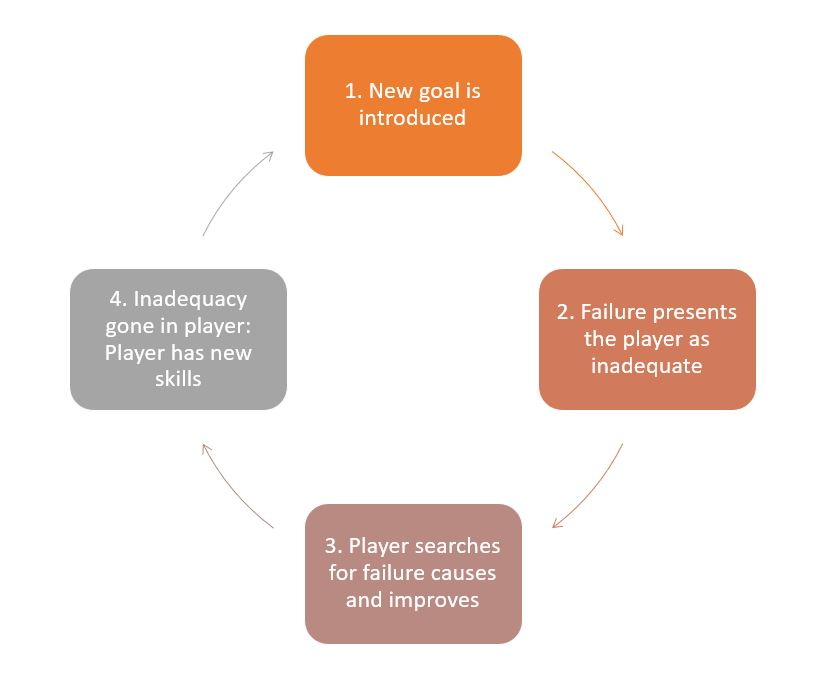
\includegraphics[width=0.5\textwidth]{figurer/Improvementcycle.JPG}}
\caption{The failure improvement cycle}
\medskip
\small\em
\label{fig:playerImprove}
\end{figure}

One of the obvious response to failure is to practice harder, but the players have a tendency to make a less obvious choice  as a response to this failure. The behavior is called \textit{``Self-Defeating behavior"} and is a way to avoid being measured and are generally unproductive. Failure makes us search for a course, a reason why and which we can attribute to our failure. It is easier to attribute our failure on other things than the lack of abilities, but to more trivial things such as lack of sleep. In games this is often done by state things such as \textit{``I did not try that hard.}, and there by making failure less painful.\cite[P.~63]{TheArtOfFailure}

There are also some players who share their most spectacular failures. These players are acting self-defeating by among other things not pursuing the official goal of the game. They are in a way creating a new goal for themselves. Self-defeating behavior and spectacular failures are two strategies which can make failure feel less negative. Games are great generators of motivation and learning. Game designers have found many ways to motivate and reward the players on. \cite[P.~64, P.~118]{TheArtOfFailure}





%\begin{figure}[h!]
   %\centering
%   \makebox[\textwidth][c]{\includegraphics[width=1\textwidth]{figurer/totalBak.png}}
%  \caption{Oversikt over totalt antall gjenlevende bakterier i biofilm med behandling av Tetracyclin og Ciprofloxacin telt på blodskål. Det vises ulike konsentrasjonsnivåer av Tetracyclin og Ciprofloxacin samt en kontroll uten anitbiotikabehandling.}
%   \medskip
%  \small\em
%  \label{fig:TotalBak}
%\end{figure}

